\documentclass[10pt]{beamer}

\usetheme{metropolis}
\usepackage{appendixnumberbeamer}

\usepackage{booktabs}
\usepackage[scale=2]{ccicons}
\usepackage{mathtools}% Loads amsmath


\usepackage{pgfplots}
\usepgfplotslibrary{dateplot}

\usepackage{xspace}
\newcommand{\themename}{\textbf{\textsc{metropolis}}\xspace}

\usepackage{caption}
\usepackage{subcaption}

%1st slide
\title{Lag Penalized Weighted Correlation (LPWC)}
\date{}
\author{Thevaa Chandereng, Anthony Gitter}

\begin{document}

\maketitle

% 2nd slide
\begin{frame}{Biological Time Series}

\begin{figure}
  \centering
    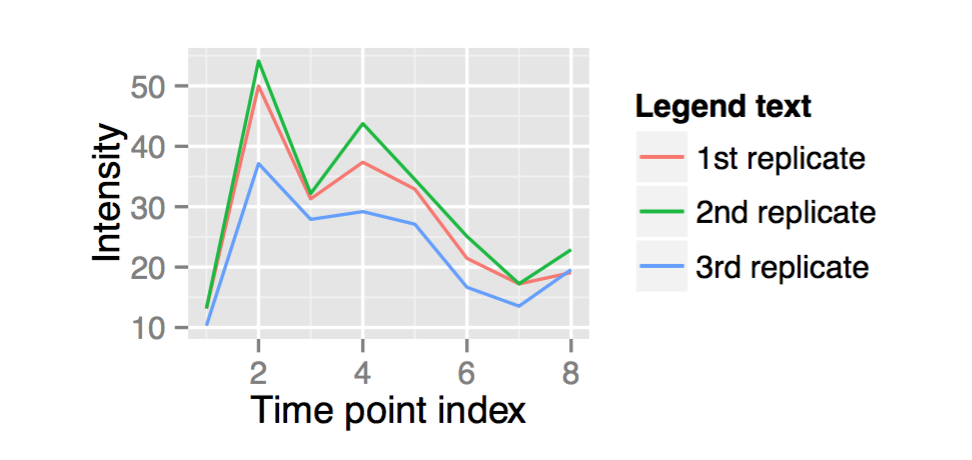
\includegraphics[width=1.0\textwidth]{Timeseries.png}
  \caption{Simple time series plot with 8 time points and 3 replicates}
\end{figure} 
   
\end{frame}


% 3rd slide
%\begin{frame}{Biological Time Series}
%    
%\begin{itemize}
%\item Snapshot of biological functions over time
%\item Study complex and dynamic biological systems 
%\item Tracking levels of genes/proteins reveals interactions
%\item Biological time series are shorter compared to time series data in other domains (5-30 time points)
%\item Similarity in temporal behavior may correspond to similarity in biological processes 
% \end{itemize}
%
%\end{frame}

%\begin{frame}{Types of Clustering Algorithms}
%    \begin{figure}
%    \centering
%        \begin{subfigure}{.5\textwidth}
%          \centering
%          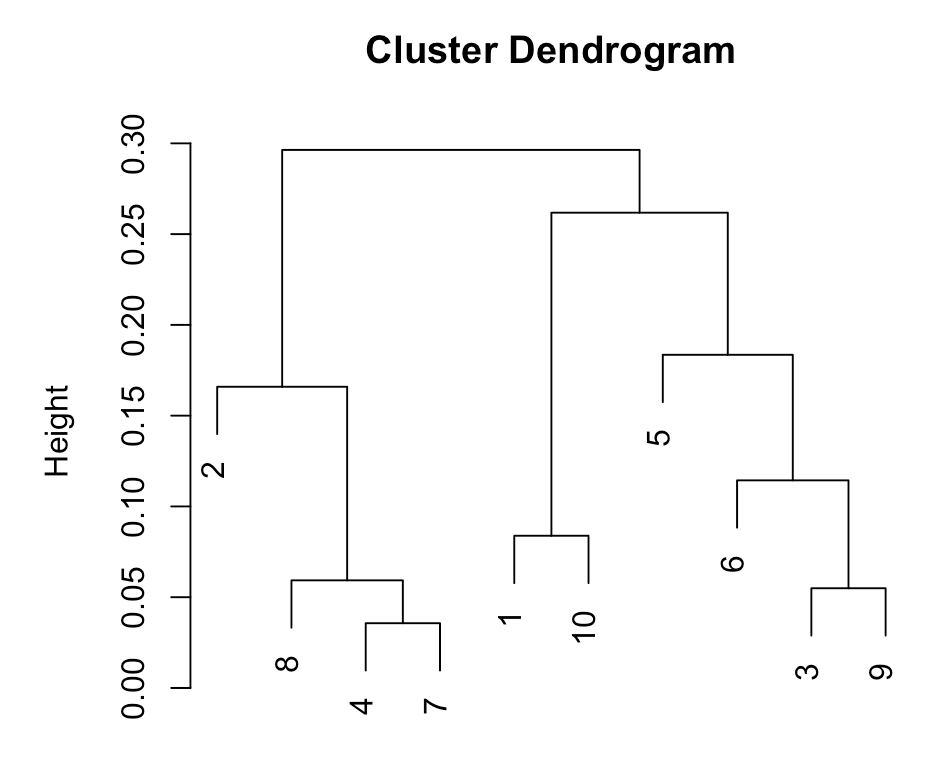
\includegraphics[width=1\linewidth]{hclust.png}
%          \caption{Hierarchical-based clustering}
%          \label{fig:sub1}
%        \end{subfigure}%
%        \begin{subfigure}{.5\textwidth}
%          \centering
%          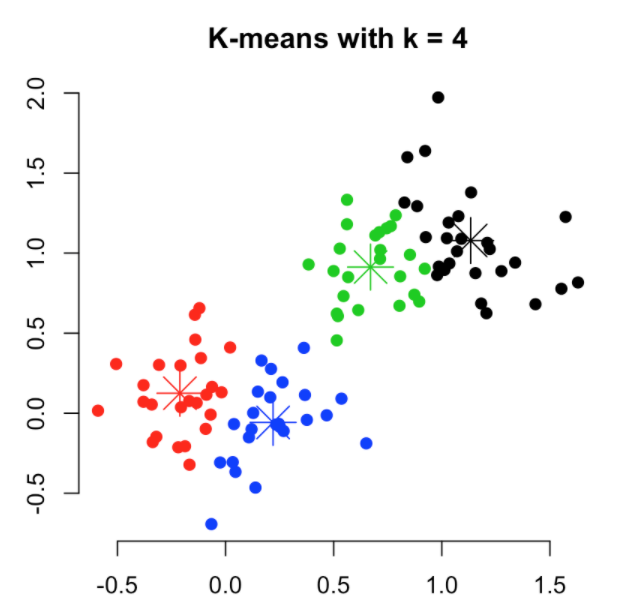
\includegraphics[width=1\linewidth]{partition.png}
%          \caption{Partition-based clustering. Image adopted from R package vignette factoextra.}
%          \label{fig:sub2}
%        \end{subfigure}
%    \caption{Two different clustering strategies}
%    \label{fig:test}
%    \end{figure}
%\end{frame}



\begin{frame}{Toy Example: Intuitive Clustering}
    \begin{figure}
     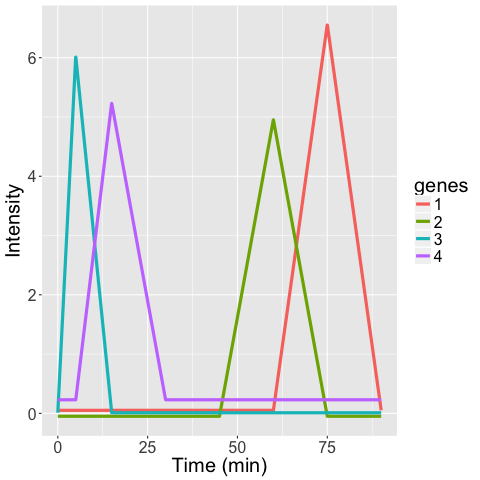
\includegraphics[width=0.5\linewidth]{Toy.png}
      \caption{Hypothetical example with 4 genes}
       \label{fig:sub11}
    \end{figure}
\end{frame}



\begin{frame}{Toy Example: Algorithmic Clustering}
    \begin{figure}
    \centering
        \begin{subfigure}{.5\textwidth}
          \centering
          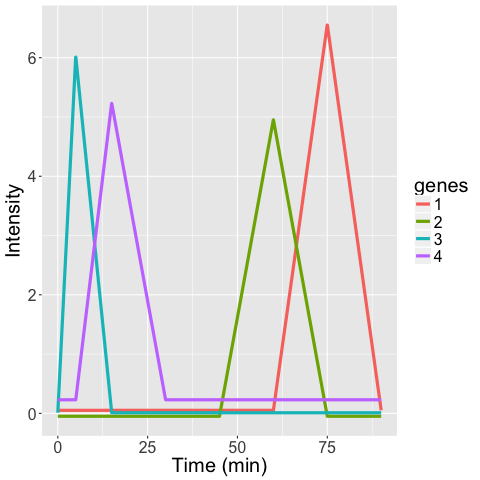
\includegraphics[width=1\linewidth]{Toy.png}
          \caption{Hypothetical example with 4 genes}
          \label{fig:sub1}
        \end{subfigure}%
        \begin{subfigure}{.5\textwidth}
          \centering
          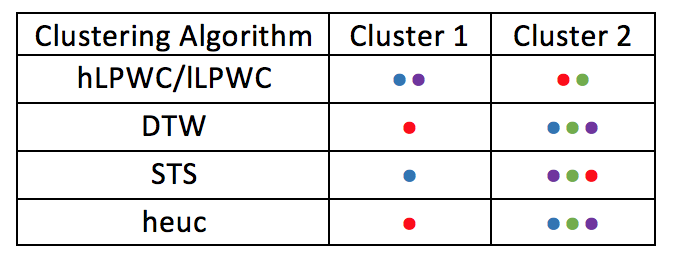
\includegraphics[width=1\linewidth]{TableCluster.png}
          \caption{Cluster assignment of the 4 genes}
          \label{fig:sub2}
        \end{subfigure}
    \caption{Existing methods do not group early and late genes}
    \label{fig:test}
    \end{figure}
\end{frame}

\begin{frame}{Motivation}
Irregular time sampling

\begin{figure}
     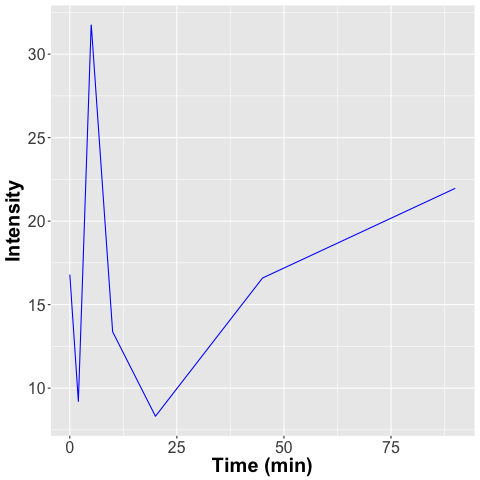
\includegraphics[width=0.6\linewidth]{sample.png}
      \caption{Irregularly sampled time series data}
       \label{fig:irregular}
    \end{figure}

\end{frame}


\begin{frame}{Motivation}
Delayed response (lags)

\begin{figure}
     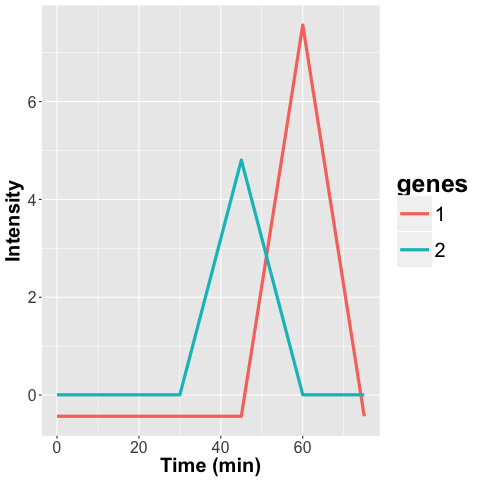
\includegraphics[width=0.5\linewidth]{delay.png}
      \caption{Gene 1 spikes after gene 2}
       \label{fig:irregular}
    \end{figure}

\end{frame}



\begin{frame}{What is a Lag?}
\begin{figure}
     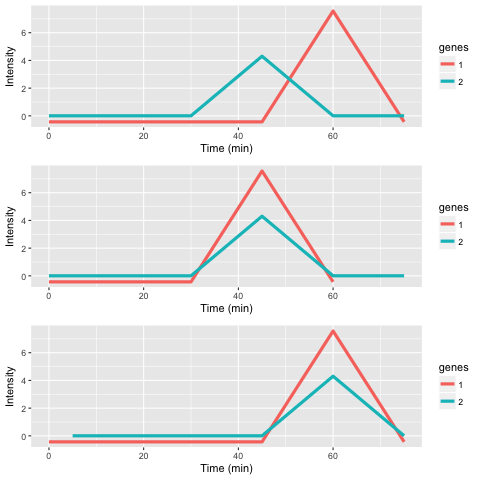
\includegraphics[width=0.60\linewidth]{Lags.png}
      \caption{An example of the effects of applying different lags to genes 1 and 2.  Gene 1 and 2 are not lagged in top row. Gene 1 with lag 1 i }
       \label{fig:lags}
    \end{figure}

\end{frame}


\begin{frame}{Method Overview}
LPWC is composed of two steps:
\begin{itemize}
\item computing optimal lags for each gene
\item computing final correlation matrix for all gene
\end{itemize}

General Formula


\begin{multline*}
corr_{LPWC}(i, j, X_i, X_j) = \underbrace{exp(\frac{- E(w)}{C})}_{\text{penalty}}  * 
\underbrace{corr_w(L^{X_i}Y_i, L^{X_j}Y_j, exp(\frac{- w}{C}))}_{\text{weigthed correlation}}
\end{multline*}
\end{frame}

\begin{frame}{Algorithm}
\textbf{Computing optimal lag}

$$score_{j} = \underset{X_i \in \{-m,..., m\}}{\mathrm{max}} \;\, corr_{LPWC}(i, j, X_i, 0) \quad \forall j \neq i$$

$$lag_{j} = \underset{X_i \in \{-m,..., m\}}{\mathrm{arg \,max}} \;\, corr_{LPWC}(i, j, X_i, 0) \quad \forall j \neq i$$
Then, a best lag $\hat{X}_i$ for gene $i$ assigned by 
\[
\hat{X}_i = \underset{k \in \{-m, ..., m\}}{\mathrm{arg \,max}} \sum_{j \neq i} I(lag_j = k) * score_j
\]

This is repeated to select a best lag for all genes.

\textbf{Computing final correlation matrix}
\begin{multline*}
 corr_{LPWC}(i, j, \hat{X}_i, \hat{X}_j) = 
exp(\frac{- E(w)}{C}) * corr_w(L^{\hat{X}_i}Y_i, L^{\hat{X}_j}Y_j, exp(\frac{- w}{C}))
\end{multline*}
\end{frame}

\begin{frame}{Existing Time Series Clustering Methods}
Partition-based
\begin{itemize}
\item Short Time-series Expression Miner (STEM)
\item Graphical Query Language (GQL)
\item Cluster Analysis of Gene Expression Dynamics (CAGED)
\end{itemize}

Hierarchical-based
\begin{itemize}
\item Dynamic Time Warping (DTW)
\item Short Time Series Distance (STS)
\end{itemize}
\end{frame}


\begin{frame}{Clustering Accuracy}
\begin{itemize}
\item  Adjusted Rand Index (ARI): similarity between two data clusterings and adjusted for chance 
\item  ARI score close to 1 indicates similar clusterings, score close to 0 otherwise
\end{itemize}
\end{frame}


\begin{frame}{Simulated Data}
\begin{figure}
     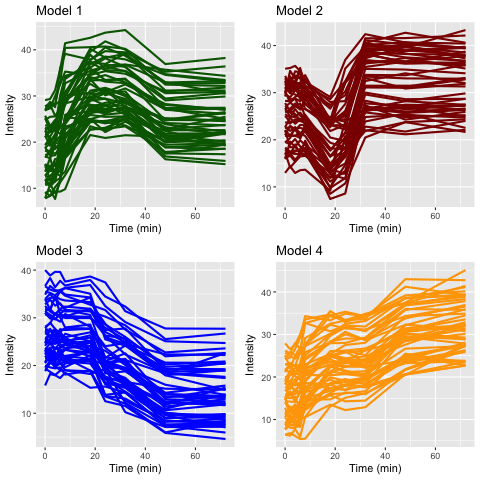
\includegraphics[width=0.65\linewidth]{Simulation_plot.png}
      \caption{Four models simulated using ImpulseDE. Random noise was added to the model parameters to induce variation around a common trend.}
       \label{fig:simdata}
    \end{figure}
\end{frame}



\begin{frame}{ARI Score for Simulated Data}
\begin{figure}
     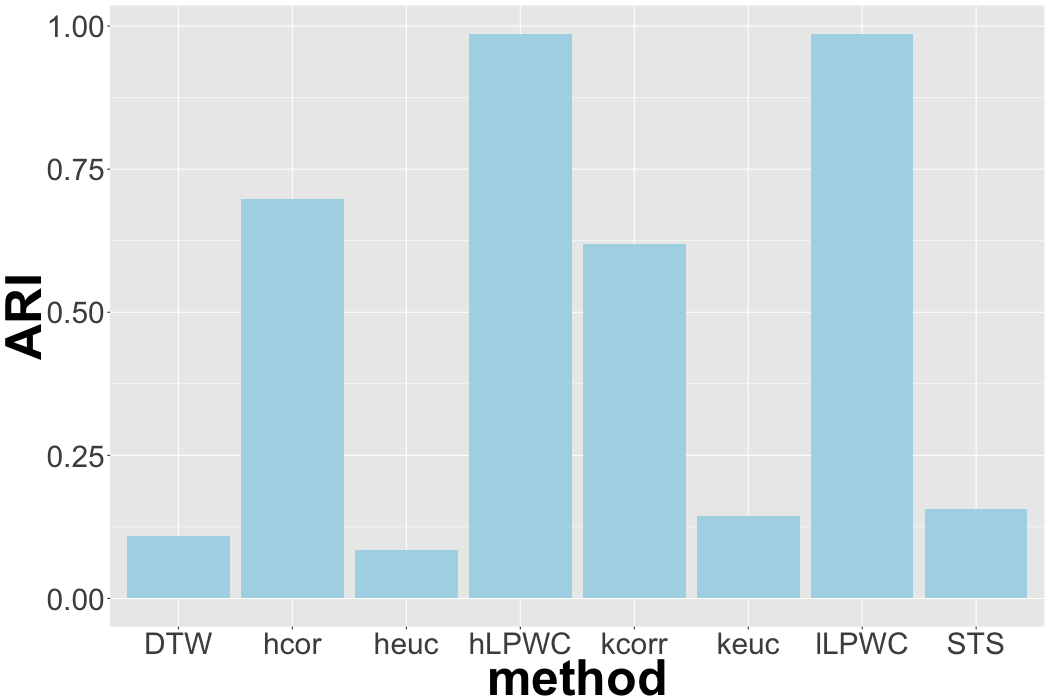
\includegraphics[width=0.7\linewidth]{ARI-Impulse.png}
      \caption{ARI score for different clustering methods for the simulated data where the real clusters are known.}
       \label{fig:ariscore}
    \end{figure}

\end{frame}



\begin{frame}{Yeast Osmotic Stress Response Data}
\begin{figure}
     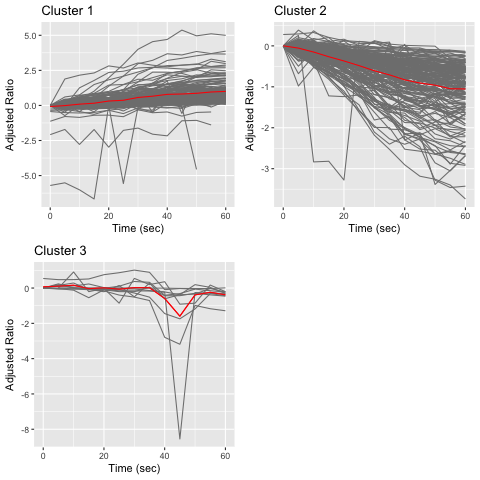
\includegraphics[width=0.65\linewidth]{yeast_cluster_lLPC.png}
      \caption{Clustering 344 phosphopeptides in yeast osmotic stress into 3 different clusters. }
       \label{fig:ariscore}
    \end{figure}

\end{frame}




\begin{frame}{Conclusion \& Future Work}
\begin{itemize}
\item Algorithm tackles the issue of irregular time samples and delayed responses
\item Preference for distance-based or correlation-based clustering is subjective
\item R package available on CRAN (LPWC) and preprint on bioRxiv
\item Allow missing data (imputation) and support mixed dataset with different time points
\item Improve the optimal lag assignments
\end{itemize}
\end{frame}


\begin{frame}{Acknowledgements}

\begin{itemize}
\item Ron Stewart, Karl Broman, James Dowell, Wenzhi Cao, Jen Birstler, and members of Gitter lab
\item Funding from the NSF and UW Carbone Cancer Center
\end{itemize}

\end{frame}



%end
\end{document}
